\documentclass[conference]{IEEEtran}
\usepackage{amsmath,amssymb,amsfonts}
\usepackage{url}
\usepackage{hyperref}
\usepackage{fullpage}

\usepackage{fancyvrb}
\newtheorem{lemma}{Lemma}
\usepackage{graphicx} % Required for inserting images
\usepackage[backend=biber,
style=numeric]{biblatex}
\addbibresource{citations.bib}

\title{Evaluating Performance Differences in Two Shortest-Path Finding Algorithms}
\author{Alec Olson \\ ols00160@umn.edu \\ November 24, 2025}
\date{November 24, 2025}

\begin{document}

\maketitle

\section{History}
Shortest-path finding algorithms are ubiquitous in the world around us. Many people rely on popular map apps that implement these algorithms, such as Google Maps and Apple Maps, to assist them with navigation as they drive to unfamiliar destinations. The algorithms are also widely used in routing internet and phone traffic, informing robots how to move, and designing routes for delivery drivers who must make multiple stops (colloquially referred to as the Traveling Salesman Problem). This paper will not examine this last point because it is significantly more complicated than simply finding the fastest route between two points, but it provides an interesting and compelling example of an extension of the topics discussed here.
\newline
\newline
In 1959, Edsgar Dijkstra published a paper titled, “A Note on Two Problems in Connexion with Graphs,” where he outlined an algorithm for finding the shortest path between two nodes in a graph \cite{dijkstra_note_1959}. Over time, this came to be known as Dijkstra’s Algorithm. Less than a decade later, in 1967, Peter Hart, Nils Nilsson, and Bertram Raphael published a paper titled, “A Formal Basis for the Heuristic Determination of Minimum Cost Paths,” where they described a new algorithm, which they called A*, that was designed similarly to Dijkstra’s but with one key difference. The A* Algorithm was aided by the use of a heuristic function that estimates the cost between a given node and the goal node. This heuristic function improves the algorithm’s ability to guess at what the next-best node in the path is, which generally allows A* to calculate the optimal shortest path more quickly than Dijkstra’s Algorithm. 

\section{Goal of this Project}
To empirically measure performance differences between different implementations of two different shortest-path finding algorithms applied to a network of roads in the Twin Cities metro area: Dijkstra’s and A*.
\newline
\newline
I built a program to find the fastest driving route between two intersections in the Twin Cities metro area. In essence, it is a greatly simplified version of Google Maps. I used a dataset of roads from the Minnesota Geospatial Commons \cite{MetroGIS}. My GitHub repository is linked in the References section \cite{github}.

\section{Description of Dijkstra's Algorithm}
\begin{enumerate}
    \item Construct a graph $(V, E)$ of vertices and edges. The graph can be either directed or undirected. However, one important point is that it cannot have negatively-weighted edges. For most real-world applications, this is not a problem because costs in the real-world are almost exclusively positive. However, since the algorithm tries to find the path with lowest cost, a graph with negatively-weighted edges could cause the algorithm to loop through these edges indefinitely, generating ever lower and lower-cost paths.

    \item Select a starting node $v_s$ and a goal node $v_g$.

    \item Each vertex stores information about the cost to reach that vertex from $v_s$. Initially, set this value to infinity for all vertices except for $v_s$, whose cost will be zero. Dijkstra's Algorithm works by iteratively minimizing the cost to reach a given vertex, which is why we want to have a starting cost for each vertex to be infinity.

    \item Create a set of all the vertices that have not been visited. Initially, this set is equal to $V$ because no vertex has been visited by the algorithm. Call this set $U$.

    \item Select a vertex $v$ from $U$ that has the lowest cost. For the first iteration of this algorithm, this vertex is the $v_s$ because it has cost 0, and every other vertex has cost infinity.

    \item If $v$ equals $v_g$, then Dijkstra’s Algorithm has successfully found a path.

    \item Examine the neighbors of $v$. This step is called $expanding$ $v$. Its neighbors are the vertices that are directly connected to $v$ by one edge.

    \begin{itemize}
        \item For each neighbor $n$ of $v$, update its cost. Its new cost is equal to $v$’s cost + the cost of the edge between $v$ and $n$. This new cost represents the total cost to reach $n$ from $v_s$.

    \end{itemize}

    \item Remove $v$ from $U$.

    \item Repeat steps 5 through 8 until one of two things has happened:

    \begin{enumerate}
        \item The algorithm reaches $v_g$, in which case it has found a lowest-cost path.

        \item $U$ becomes empty, in which case the algorithm has visited every vertex but has not found a path to $v_g$. The algorithm fails in this scenario. However, if the graph is connected (that is, every vertex can reach every other vertex), then the algorithm will always find a solution.
    \end{enumerate}

\end{enumerate}


\section{Description of the A* Algorithm}
The A* Algorithm works much the same as Dijkstra’s Algorithm. The main difference is in how it selects the next vertex to examine during each iteration of the algorithm. Given a starting vertex $v_s$ and a goal vertex $v_g$, the algorithm calculates two values for each vertex $v$ that it examines:
\begin{enumerate}
    \item The cost to reach $v$ from $v_s$. Label this value $g(v)$. This is the same as in Dijkstra’s Algorithm.

    \item The estimated cost to reach $v_g$ from $v$. Label this value $h(v)$. This estimate is calculated through the use of a heuristic function. This function is the key difference between Dijkstra’s Algorithm and the A* Algorithm, and the success of the A* Algorithm depends on choosing a good heuristic function.

\end{enumerate}

Then, each vertex stores an $f$ value calculated as follows:
\[f(v) = g(v) + h(v)\]
This $f$ value allows the A* algorithm to be informed while it is searching for the lowest-cost path. Nodes that are closer to being on this path will have a lower $f$ value, and nodes that are far away from the path will have a higher $f$ value.
\newline
\newline
During each iteration, the A* Algorithm chooses to examine the vertex with the lowest $f$ value. If the heuristic function $h$ is designed properly, the use of $f$ allows the algorithm to more quickly find a lowest-cost path because it prioritize searching nodes that are on or near this path instead of investigating extraneous nodes in vain.

\subsection{Designing the Heuristic Function}
There are two characteristics of a good heuristic function $h$:
\begin{enumerate}
    \item \textbf{Admissibility}: A heuristic function is said to be admissible if it never overestimates the true cost between $v$ and $v_g$. Let $c$ be a function that returns the true cost between a given vertex and $v_g$. Then, expressed formally, $h$ is admissible if:
    \[\forall v \in V: \ h(v) \leq c(v)\]

    \item \textbf{Consistency}: A heuristic function is said to be consistent if it never overestimates the sum of the true cost between two vertices $v_1$ and $v_2$ in the graph and the estimate of reaching $v_g$ from $v_2$. Let $c$ be a function that returns the true cost between two vertices. Then, expressed formally, $h$ is consistent if:
    \[\forall v_1, v_2 \in V: \ h(v_1) \leq c(v_1, v_2) + h(v_2)\]

\end{enumerate}

All heuristic functions that are consistent are also admissible, but the inverse is not always true. If the heuristic function is admissible, then the A* Algorithm will always return an optimal shortest-cost solution \cite{hart_formal_1968}. 

\subsection{Designing my Heuristic Function}
Designing a heuristic function for a road network is relatively simple, but there is one important point that must be carefully considered.
\newline
\newline
For a road network that spans just a few counties in the Twin Cities metro area, it is permissible to ignore the curvature of the Earth’s surface. Therefore, we can describe the road network as existing in a two-dimensional Euclidean plane. The roads become line segments, and the intersections are points.
\newline
\newline
The cost between two intersections is defined as the time necessary to travel in a car between them. Therefore, the first component of designing the heuristic function for this application is estimating the distance between two intersections. The shortest distance between any two points $(x_1, y_1)$ and $(x_2, y_2)$ is defined by the Euclidean distance: \[d = \sqrt{(x_1 - x_2)^2 + (y_1 - y_2) ^ 2}\]
This distance will never overestimate the true distance between any two intersections in the road network because it is the shortest possible distance between two points in Euclidean space.
\newline
\newline
The second component of designing the heuristic function is to estimate the travel time between two intersections. Given a distance $d$ and a speed $s$, time is calculated as follows: 
\[t = \frac{d}{s}\]
This is the part where it is vital to carefully consider how to estimate the time to travel along a given road segment. Each road segment has a different speed limit. In order to design a heuristic that never overestimates the cost to travel between two intersections, it is vital to select $s$ such that it is the maximum possible speed limit in the road network.
\newline
\newline
For example, in the data for the Twin Cities, the maximum speed limit on any road is 70 mph. Therefore, I set $s = 70$. Using $d$ as calculated above, we then obtain a value for $t$ that will never overestimate the true cost of travel between two intersections. The value of $t$ is used as the output for my heuristic function.
\newline
\newline
Of course, this is assuming that cars never drive faster than the speed limit. In reality, they do this all the time, but for this project, I assume that speed limits are strictly adhered to.
\newline
\newline
The distance of a road between any two intersections is strictly less than or equal to the Euclidean distance between the intersections, and the speed limit on all the roads is no faster than 70 mph. Let $c$ be a function that returns the true cost between two nodes. Then, for every node $n$, with an intermediate node $n'$ which is somewhere on the path between $n$ and the goal node $v_g$, \[h(n) \leq c(n, n') + h(n')\] 
This means that my heuristic function is consistent, which means that it is also admissible. Therefore, my implementation of A* will generate an optimal solution.


\section{My Implementation of A*}
We must first create a graph of the road network in an efficient way, where the nodes are intersections and the edges are road segments. The graph is best stored as a hash table, where each key is an intersection, and each value is a Node object, which stores information about each intersection. Node objects are described below.
\newline
\newline
It is important to store the graph as a hash table in order to ensure $O(1)$ lookup. For example, the dataset for Hennepin County has around 35,000 intersections, so it is imperative to design the graph efficiently.
\newline
\newline
I define two classes to store information about each intersection. One class, called $Vertex$, stores three attributes:
\begin{itemize}
    \item \textit{index}: A reference to more data about this object in a database.

    \item \textit{neighbors}: Information about which vertices neighbor this vertex.

    \item \textit{coordinates}: The coordinates of this vertex in UTM15N. This coordinate system uses meters instead of degrees. Using meters allows for easy distance calculations between two vertices.

\end{itemize}
Objects of this class are immutable and are generated during the expansion of nodes in the A* algorithm.
\newline
\newline
The other class is called $Node$. $Node$ objects are the values of the hash table described above. One $Node$ object is generated for each intersection. These objects store the following attributes:
\begin{itemize}
    \item \textit{visited}: A boolean value that keeps track of whether the A* Algorithm has visited this intersection. This value is initially $False$ for all nodes.

    \item \textit{cost}: A way to store the current lowest cost to travel to this intersection from the starting intersection. This value is initially $\infty$ for all nodes except for the starting node, which is initialized to $0$.

    \item \textit{f}: This attribute stores the $f$ value of each node. Remember, $f$ is calculated as follows:
    \[f(n) = g(n) + h(n)\]
    where $g$ is the true cost between the starting node and the given node, and $h$ is the estimated cost between the given node and the goal node.

    \item \textit{prev}: Initialized to $null$, this attribute will be updated once the given node has been added to a path. It stores a pointer to the previous node in the path, which can then be used to construct the full path once the A* Algorithm returns.

    \item \textit{neighbors}: Information about which vertices neighbor this vertex.

    \item \textit{coordinates}: The coordinates of this vertex in UTM15N. This coordinate system uses meters instead of degrees. Using meters allows for easy distance calculations between two vertices.
    
\end{itemize}

information about whether A* has visited the intersection; the current best cost to reach the intersection from the starting node; the node’s $f$ value (the current best cost to reach the intersection + the heuristic function's output, which is the estimate to reach the goal node from this node); a pointer to the previous intersection in the route (used to build the final route once A* returns); a reference to the neighboring vertices of the node; and the nodes coordinates, which are used to calculate the distance between two nodes.
\newline
\newline
Note: although the objects themselves are immutable, A* may generate multiple (duplicate) Node objects for the same intersection during the expansion phase.
\newline
\newline
The A* function takes as its parameters the road network and two $Vertex$ objects, one containing information about the starting intersection and the other containing information about the goal intersection.
\newline
\newline
A* proceeds as follows:
\begin{enumerate}
    \item Add to a minimum binary heap the $Vertex$ object that refers to the starting intersection.

    \item While the heap is not empty:

    \begin{enumerate}
        \item Extract the $Vertex$ object which has the lowest $f$ value. Remember, $f$ is defined as:
        \[f(x) = g(x) + h(x)\]
        where $g$ is the current lowest cost between the starting node and the current node, and $h$ is the estimated cost to travel from the current node to the goal node.

        \item If this $Vertex$ object corresponds to the goal intersection, return the road network. Using the attribute of each $Node$ that stores information about the previous $Node$ in its path, it is possible to construct the optimal shortest-path solution.

        \item If the $Vertex$ object does not correspond to the goal intersection, expand it.

        \begin{enumerate}
            \item Create a new $Vertex$ object for each neighboring intersection.

            \item Update these $Vertex$ objects’ cost and $f$ attributes

            \item If these intersections haven’t been visited before AND their new $f$ value is lower than their old $f$ value, then push the object onto the heap. Update its $prev$ attribute accordingly.

        \end{enumerate}

        \item Mark the $Vertex$ object as visited.

    \end{enumerate}

    \item Starting with the goal intersection, use the $prev$ attributes of each $Node$ object to determine the final path.

\end{enumerate}


\section{My Implementation of Dijkstra's Algorithm}
My implementation of Dijkstra's Algorithm is almost identical to my implementation of the A* Algorithm. The only difference is the omission of the heuristic function to better inform the search process.


\section{Runtime Evaluation}
In the naive implementation of a shortest-path finding algorithm, the nodes are all stored in an immutable, unsorted array. Then, each iteration of the algorithm must perform a linear search through the array to find the node with lowest cost. This is highly inefficient. The worst-case runtime of an algorithm that takes this approach is $O(v^2)$, where $v$ is the number of vertices. In the worst-case scenario, the algorithm must visit every vertex, and for each visit, it must completely iterate through the array, which has length $v$.
\newline
\newline
In a dataset containing just Hennepin County, there are approximately 35,000 nodes. The algorithm typically takes thousands of iterations to find a solution, meaning that it must perform millions of operations to search through the array and find the vertex with minimum cost.
\newline
\newline
Instead, it is wise to store the nodes in a minimum binary heap. A minimum binary heap is a binary tree in which each parent has a value that is smaller than its children. Given $n$ nodes in the heap, storing the nodes in this data structure allows $O(log_2(n))$ extraction. Finding the minimum node is accomplished in $O(1)$ time, and then reorganizing the heap to maintain its minimum property runs in $O(log_2(n))$ time. The worst-case runtime of an algorithm that takes this approach is $O(v * log_2(v))$, where $v$ is the number of vertices. In the worst-case scenario, the algorithm must visit every vertex, and for each visit, it will spend $O(log_2(v))$ time extracting the minimum vertex from the heap.
\newline
\newline
When working with large datasets that have tens of thousands of nodes, the algorithm that runs in $O(v * log_2(v))$ time will perform significantly faster than an algorithm that runs in $O(v^2)$ time.
\newline
\newline
There are two possible implementations of these shortest-path finding algorithms as far as minimum binary heaps are concerned.
\begin{enumerate}
    \item Before the algorithm begins, add all the vertices to the heap. After a vertex is visited, remove it from the heap and reorganize the heap to maintain its minimum binary property.

    \item Before the algorithm begins, create a heap that contains only one element: the starting vertex. When each vertex is visited, add its neighbors to the heap. After a vertex is visited, remove it from the heap and reorganize the heap to maintain its minimum binary property.
    
\end{enumerate}
Binary heap algorithms like extracting the minimum value and pushing a node onto the heap run in $O(log_2(n))$ time. When working on datasets that have tens of thousands of nodes in their graphs, the performance improvements compared to the naive, immutable, unsorted array approach are significant.
\newline
\newline
The second approach has a strong advantage compared with the first approach. Its advantage is that the heap will generally remain much smaller than in the first approach because nodes that are not being considered will not be pushed onto the heap. In the first approach, all the nodes are initially stored in the heap, whether or not they are used. Maintaining a smaller heap allows for faster runtimes and lower memory requirements. For this reason, my heap implementations of the shortest-path finding algorithms use the second approach.


\section{Performance Evaluation}
I implemented Dijkstra's Algorithm and the A* Algorithm with two different approaches each. The first approach uses the naive way to store nodes in the graph. That is, it stores each node in an immutable, unsorted array, and each iteration of the algorithm must perform a linear search through the array to find the node with the smallest cost. The second approach uses a minimum binary heap to store nodes, significantly reducing the time necessary to find the smallest node.
\newline
\newline
As expected, the algorithms that used a minimum binary heap to store their nodes ran faster than the algorithms that used an immutable, unsorted array. However, I was surprised by just how significant the performance differences were. Confining the dataset of roads to just those in Hennepin County, running a naive implementation of the Dijkstra and A* Algorithms took approximately 3 seconds to run, even though they only examined around 6,000 nodes. When finding more complex routes, and examining 20,000 or 30,000 nodes, the algorithms took 10 to 15 seconds on average to run.
\newline
\newline
Note: All of this was run on my personal laptop, which is a 64-bit Windows 11 machine with an Intel i7-1185G7 processor and 16 GB of RAM. That is to say, it is a standard, off-the-shelf laptop.
\newline
\newline
In contrast, the efficient implementations of the Dijkstra and A* Algorithms found optimal solutions extremely quickly. Even when finding complex paths through 20,000 or 30,000 nodes, they ran in around 0.1 seconds. This significant improvement in performance was surprising. I was expecting the more efficient algorithms to run faster, but I did not anticipate just how much better they would be.
\newline
\newline
Interestingly, the difference in runtime between the corresponding naive and efficient implementations of the Dijkstra and A* Algorithms was negligible. The naive implementations of the Dijkstra and A* Algorithms both ran within 0.5 seconds of each other, and neither was consistently faster than the other. Similarly, the efficient implementations of the Dijkstra and A* Algorithms both ran within a few hundredths of a second of each other. Again, sometimes Dijkstra was faster, and other times, A* was faster. A comprehensive analysis of hundreds or thousands of calls to these algorithms would be necessary to draw a conclusion about which algorithm is generally faster, Dijkstra or A*.
\newline
\newline
At the beginning of this project, I was planning on creating a dataset that would allow the algorithm to find a path between any two intersections in the seven-county Twin Cities area. However, I restricted the dataset to just a single county at a time (e.g. just Hennepin County or just Ramsey County) after seeing the poor runtime of the naive algorithms. Running these on the entire metro area would take an extremely long time. However, the speed with which the efficient algorithms run means that it would be reasonable to expand the dataset to the entire metro area, or perhaps even to the entire state of Minnesota, because it is likely that they would still be able to find an optimal path through this much larger search area in a reasonable amount of time.


\begin{figure}[]
    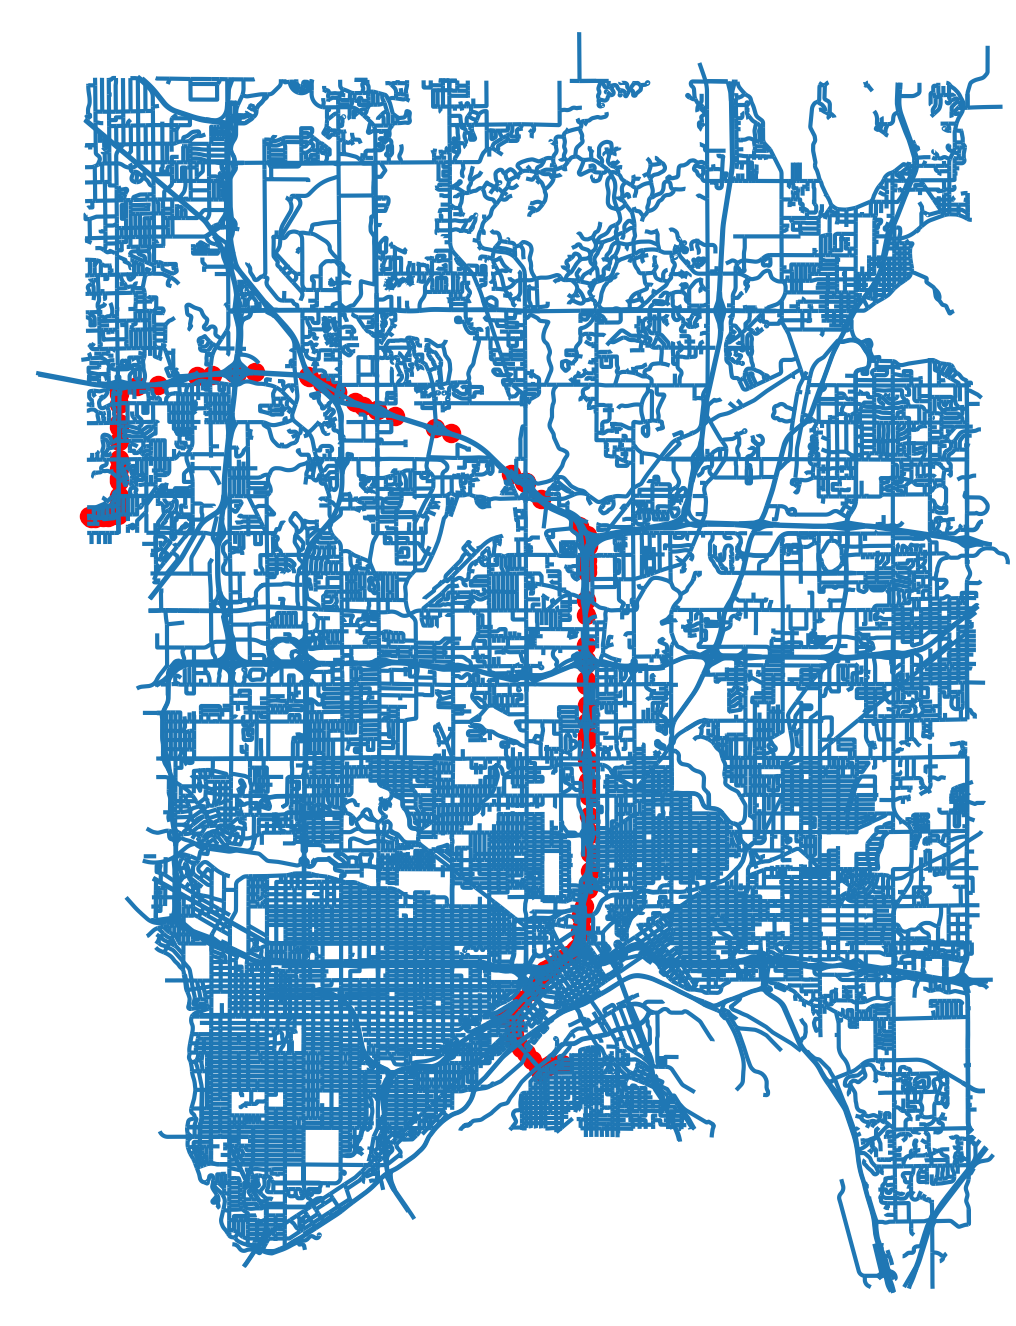
\includegraphics[width=\linewidth]{4511_proposal.png}
    \caption{An example route in Ramsey County, with the nodes (road intersections) highlighted in red and all roads in blue.}
    \label{fig:Route}
\end{figure}
\newpage


\printbibliography
% \bibliographystyle{IEEEtranN} % Specify the bibliography style here
% \bibliography{citations} % The .bib file without the extension
\end{document}

